% !TEX root = ../main.tex

\chapter{Application on historical dataset}
\label{chap:Application on historical dataset}

For purpose of demonstrating for demand I'm using data from US electricity consumption~\autocite{us-elec} It offers per month aggregation of electrical energy used per state, and for purpose of illustration I'm using whole US aggregated. Data ranges from 1990 till February 2016. I'm using restricted version from 1990 till 2005 aggregated on yearly basis. Full data plot is in figure~\ref{fig:supply}

\begin{figure}[]
  \centering
  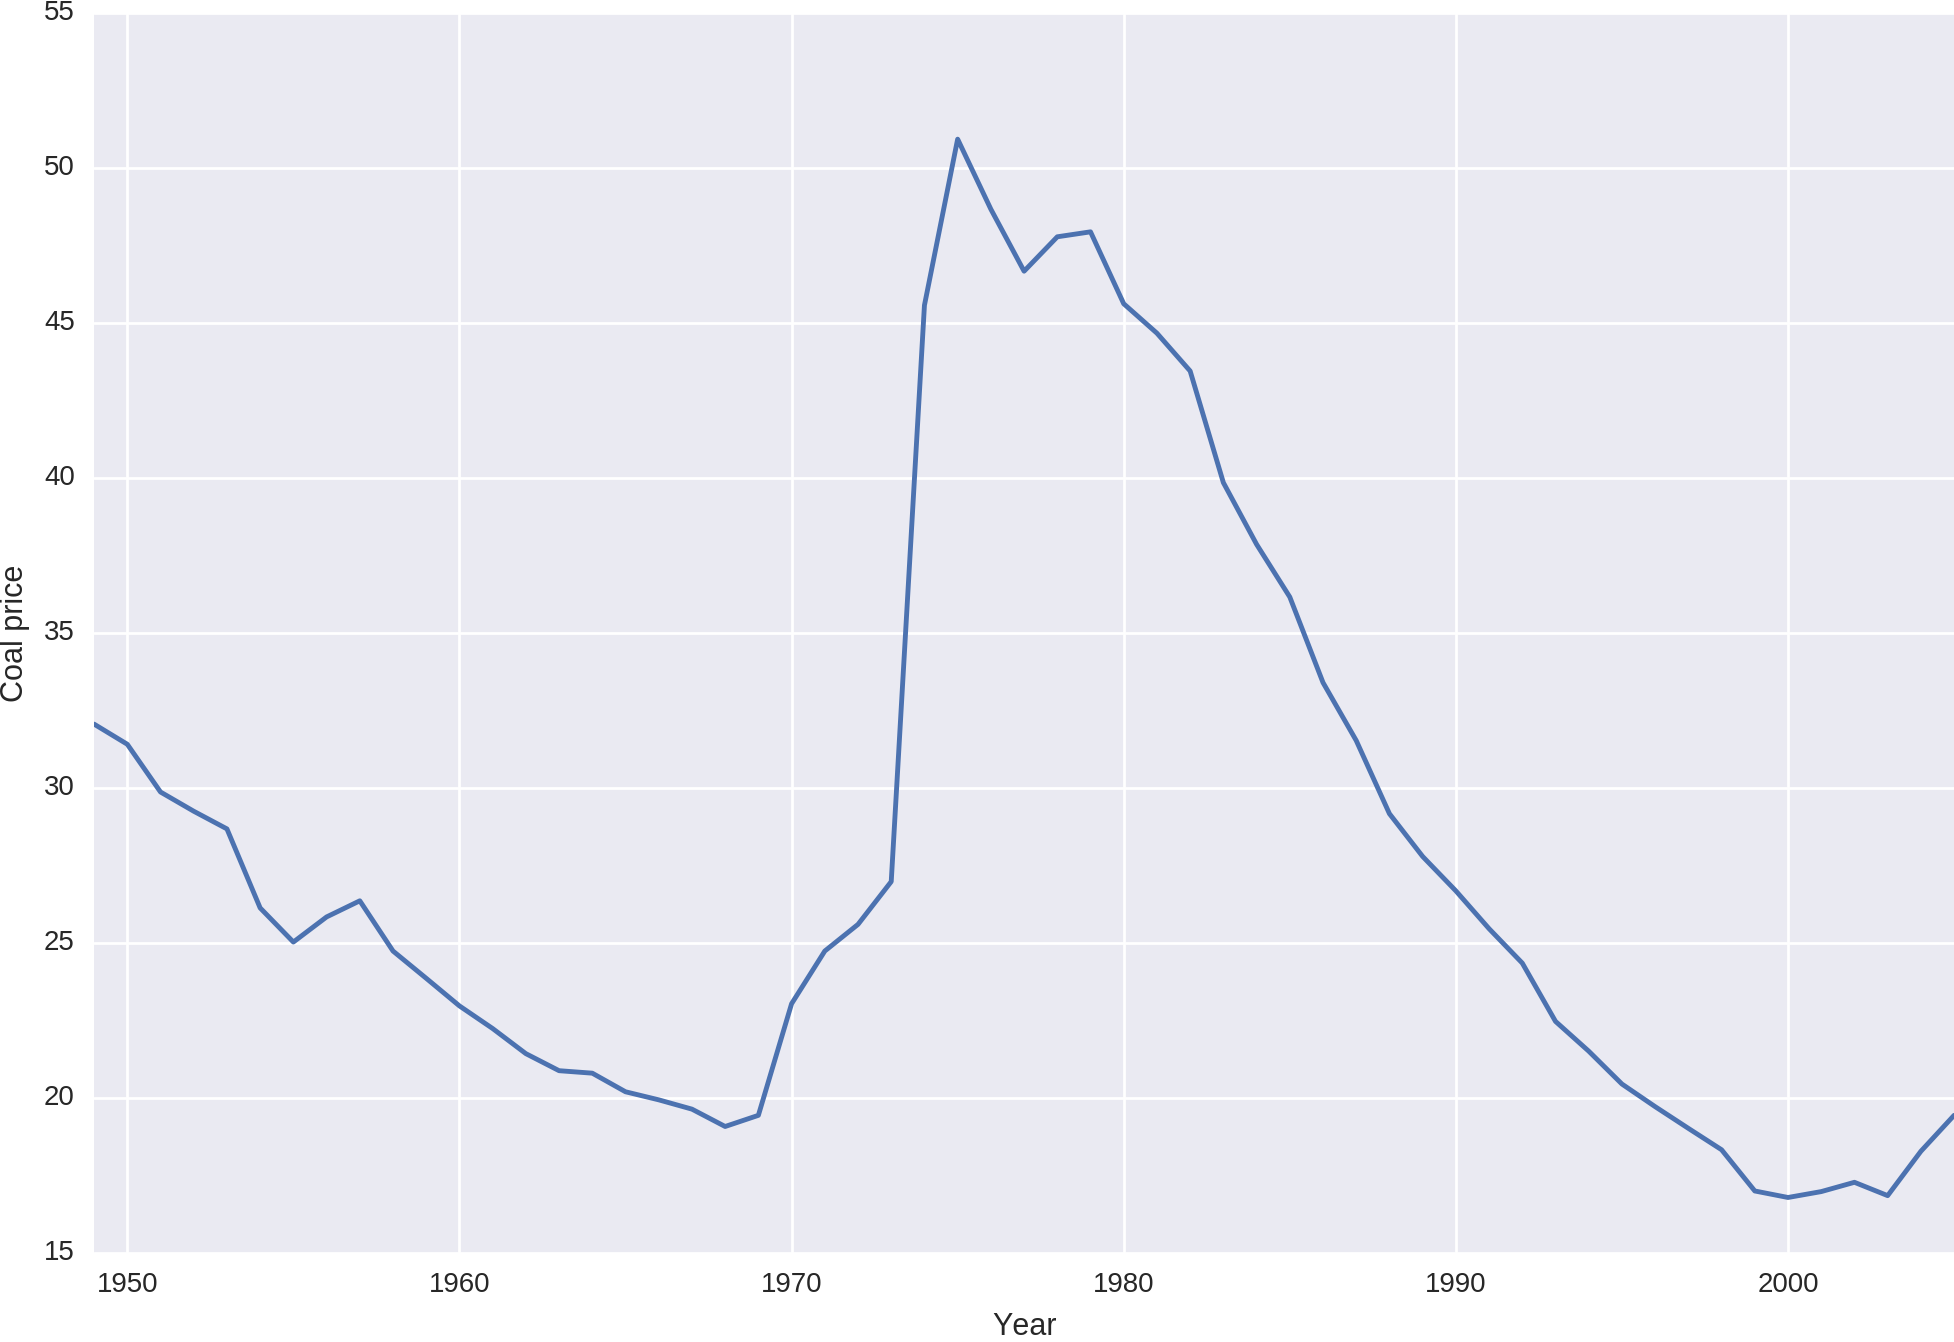
\includegraphics[width=0.8\linewidth]{supply}
  \caption{Yearly coal prices}
  \label{fig:supply}
\end{figure}

For supply unit cost, for illustrative purposes I'm using historic American coal price~\autocite{us-coal}. It is yearly based from 1950 till 2005. The data is plot is in figure~\ref{fig:demand}.

For purposes of this analysis, data from 2000 till 2005 is going to be forecasted as described in previous chapter, and then compared to ideal, perfect knowledge scenario. Analysis will be conducted for various values of $\mathbf{x_{\max}}$, $b$ and $d$ model parameters.

\begin{figure}[]
  \centering
  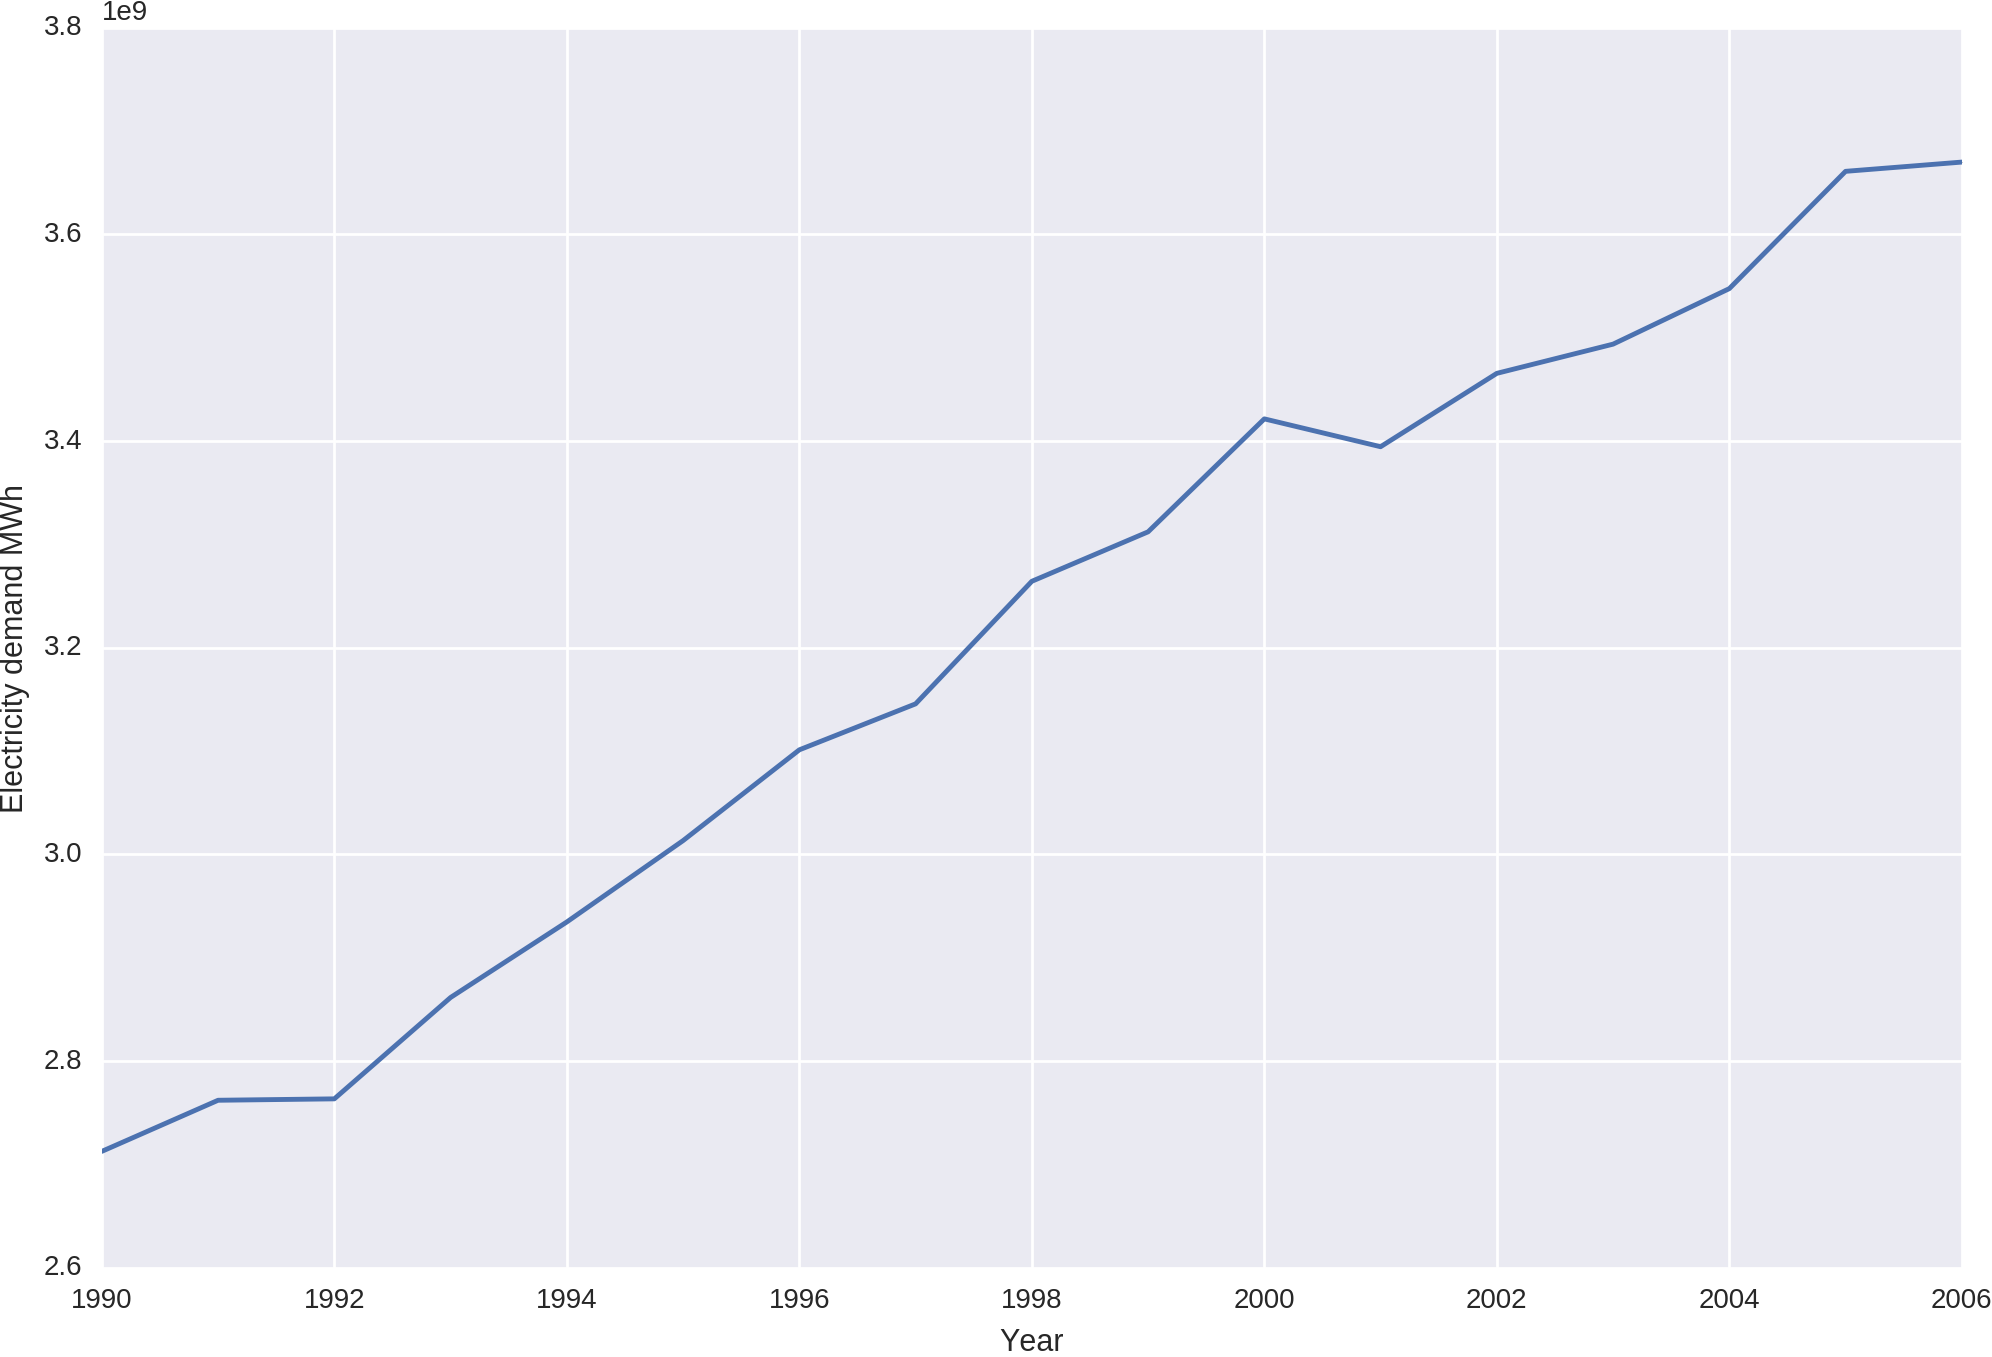
\includegraphics[width=0.8\linewidth]{demand}
  \caption{Yearly electricity demand}
  \label{fig:demand}
\end{figure}
